\documentclass{beamer}
\usepackage[utf8]{inputenc}
\usepackage{graphicx, epsfig}
\usepackage{amsmath,mathrsfs,amsfonts,amssymb}
\usepackage{floatflt}
\usepackage{epic,ecltree}
\usepackage{mathtext}
\usepackage{fancybox}
\usepackage{fancyhdr}
\usepackage{multirow}
\usepackage{enumerate}
\usepackage{epstopdf}
\usepackage{multicol}
\usepackage{algorithm}
\usepackage[noend]{algorithmic}
\usepackage{tikz}
\usepackage{blindtext}
\usetheme{default}%{Singapore}%{Warsaw}%{Warsaw}%{Darmstadt}
\usecolortheme{default}

\setbeamerfont{title}{size=\Huge}
\setbeamertemplate{footline}[page number]{}

\setbeamertemplate{section in toc}[sections numbered]


\makeatletter
\newcommand\HUGE{\@setfontsize\Huge{35}{40}}
\makeatother    

\setbeamerfont{title}{size=\HUGE}
\beamertemplatenavigationsymbolsempty

% latin bold lower
\newcommand{\ba}{\mathbf{a}} 
\newcommand{\bc}{\mathbf{c}} 
\newcommand{\be}{\mathbf{e}} 
\newcommand{\bh}{\mathbf{h}} 
\newcommand{\bp}{\mathbf{p}} 
\newcommand{\bt}{\mathbf{t}} 
\newcommand{\bs}{\mathbf{s}} 
\newcommand{\bu}{\mathbf{u}} 
\newcommand{\bv}{\mathbf{v}} 
\newcommand{\bw}{\mathbf{w}} 
\newcommand{\bx}{\mathbf{x}} 
\newcommand{\by}{\mathbf{y}} 
\newcommand{\bz}{\mathbf{z}} 

% latin bold upper
\newcommand{\bA}{\mathbf{A}} 
\newcommand{\bB}{\mathbf{B}} 
\newcommand{\bC}{\mathbf{C}} 
\newcommand{\bI}{\mathbf{I}} 
\newcommand{\bJ}{\mathbf{J}} 
\newcommand{\bL}{\mathbf{L}} 
\newcommand{\bM}{\mathbf{M}} 
\newcommand{\bP}{\mathbf{P}}
\newcommand{\bQ}{\mathbf{Q}} 
\newcommand{\bR}{\mathbf{R}} 
\newcommand{\bT}{\mathbf{T}} 
\newcommand{\bU}{\mathbf{U}} 
\newcommand{\bV}{\mathbf{V}} 
\newcommand{\bW}{\mathbf{W}} 
\newcommand{\bX}{\mathbf{X}} 
\newcommand{\bY}{\mathbf{Y}} 
\newcommand{\bZ}{\mathbf{Z}} 

% latin cal upper
\newcommand{\cF}{\mathcal{F}} 
\newcommand{\cG}{\mathcal{G}} 
\newcommand{\cI}{\mathcal{I}} 
\newcommand{\cL}{\mathcal{L}} 
\newcommand{\cM}{\mathcal{M}} 
\newcommand{\cN}{\mathcal{N}} 
\newcommand{\cS}{\mathcal{S}} 
\newcommand{\cT}{\mathcal{T}} 
\newcommand{\cW}{\mathcal{W}} 
\newcommand{\cX}{\mathcal{X}} 
\newcommand{\cZ}{\mathcal{Z}} 

% latin bb upper
\newcommand{\bbE}{\mathbb{E}} 
\newcommand{\bbI}{\mathbb{I}} 
\newcommand{\bbP}{\mathbb{P}} 
\newcommand{\bbR}{\mathbb{R}} 

% greek bold lower
\newcommand{\bepsilon}{\boldsymbol{\epsilon}} 
\newcommand{\btheta}{\boldsymbol{\theta}} 
\newcommand{\blambda}{\boldsymbol{\lambda}} 
\newcommand{\bpi}{\boldsymbol{\pi}} 
\newcommand{\bmu}{\boldsymbol{\mu}} 
\newcommand{\bsigma}{\boldsymbol{\sigma}} 
\newcommand{\bphi}{\boldsymbol{\phi}} 

% greek bold upper
\newcommand{\bSigma}{\boldsymbol{\Sigma}} 

\DeclareMathOperator*{\argmin}{arg\,min}
\DeclareMathOperator*{\argmax}{arg\,max}

\newcommand{\createdgmtitle}[1]{\title[\hbox to 56mm{Deep Generative Models  \hfill\insertframenumber\,/\,\inserttotalframenumber}]
	{\vspace{1cm} \\ Deep Generative Models \\ {\Huge Lecture #1}}
	\author{Roman Isachenko}
	\institute{
	Moscow Institute of Physics and Technology
	} 
	\date{2023, Autumn}
}

\usepackage{tikz}
\usetikzlibrary{arrows,shapes,positioning,shadows,trees}

\newcommand\myfootnote[1]{%
  \tikz[remember picture,overlay]
  \draw (current page.south west) +(1in + \oddsidemargin,0.5em)
  node[anchor=south west,inner sep=0pt]{\parbox{\textwidth}{%
      \rlap{\rule{10em}{0.4pt}}\raggedright\scriptsize \textit{#1}}};}

\newcommand\myfootnotewithlink[2]{%
  \tikz[remember picture,overlay]
  \draw (current page.south west) +(1in + \oddsidemargin,0.5em)
  node[anchor=south west,inner sep=0pt]{\parbox{\textwidth}{%
      \rlap{\rule{10em}{0.4pt}}\raggedright\scriptsize\href{#1}{\textit{#2}}}};}
      
\AtBeginSection[]
      {
      	\begin{frame}{Outline}
      		\tableofcontents[currentsection]
      	\end{frame}
      }
      \AtBeginSubsection[]{
      	\begin{frame}{Outline}
      		\tableofcontents[currentsection,currentsubsection]
      	\end{frame}
}
\createdgmtitle{8}

%--------------------------------------------------------------------------------
\begin{document}
%--------------------------------------------------------------------------------
\begin{frame}[noframenumbering,plain]
%\thispagestyle{empty}
\titlepage
\end{frame}
%=======
\begin{frame}{Recap of previous lecture}
	\vspace{-0.4cm}
	\begin{block}{Gumbel-max trick}
		Let $g_k \sim \text{Gumbel}(0, 1)$ for $k = 1, \dots, K$. Then
		\vspace{-0.3cm}
		\[
			c = \argmax_k [\log \pi_k + g_k]
		\]
		\vspace{-0.6cm} \\
		has a categorical distribution $c \sim \text{Categorical}(\bpi)$.
	\end{block}
	\vspace{-0.2cm}
	\begin{block}{Gumbel-softmax relaxation}
		{\color{violet}Con}{\color{teal}crete} distribution = {\color{violet}\textbf{con}tinuous} + {\color{teal}dis\textbf{crete}}
		\vspace{-0.2cm}
		\[
			\hat{c}_k = \frac{\exp \left(\frac{\log q(k | \bx, \bphi) + g_k}{\tau}\right)}{\sum_{j=1}^K \exp \left(\frac{\log q(j | \bx, \bphi) + g_j}{\tau}\right)}, \quad k = 1, \dots, K.
		\]
		\vspace{-0.7cm}
 	\end{block}
	\begin{block}{Reparametrization trick}
		\vspace{-0.4cm}
		\[
			\nabla_{\bphi} \mathbb{E}_{q(c | \bx, \bphi)} \log p(\bx | \be_{c} , \btheta) = \bbE_{\text{Gumbel}(0, 1)} \nabla_{\bphi} \log p(\bx | \bz , \btheta),
		\]
		where $\bz = \sum_{k=1}^K\hat{c}_k \be_k$ (all operations are differentiable now).
	\end{block}
 	\vspace{-0.2cm}
	\myfootnote{
	\href{https://arxiv.org/abs/1611.00712}{Maddison C. J., Mnih A., Teh Y. W. The Concrete distribution: A continuous relaxation of discrete random variables, 2016} \\
	\href{https://arxiv.org/abs/1611.01144}{Jang E., Gu S., Poole B. Categorical reparameterization with Gumbel-Softmax, 2016}
	}
\end{frame}
%=======
\begin{frame}{Recap of previous lecture}
	\begin{block}{Likelihood-free learning}
		\begin{itemize}
			\item Likelihood is not a perfect quality measure for generative model.
			\item Likelihood could be intractable.
		\end{itemize}
	\end{block}
	Imagine we have two sets of samples 
	\begin{itemize}
		\item $\cS_1 = \{\bx_i\}_{i=1}^{n_1} \sim \pi(\bx)$ -- real samples;
		\item $\cS_2 = \{\bx_i\}_{i=1}^{n_2} \sim p(\bx | \btheta)$ -- generated (or fake) samples.
	\end{itemize}
	Let define discriminative model (classifier):
	\[
		p(y = 1 | \bx) = P\bigl(\{\bx \sim \pi(\bx)\}\bigr); \quad p(y = 0 | \bx) = P\bigl(\{\bx \sim p(\bx | \btheta)\}\bigr)
	\]
	\vspace{-0.5cm}
	\begin{block}{Assumption}
		Generative distribution $p(\bx | \btheta)$ equals to the true distribution $\pi(\bx)$ if we can not distinguish them using discriminative model $p(y | \bx)$. \\
		It means that $p(y = 1 | \bx) = 0.5$ for each sample $\bx$.
	\end{block}
\end{frame}
%=======
\begin{frame}{Recap of previous lecture}
	\begin{itemize}
		\item \textbf{Generator:} generative model $\bx = G(\bz)$, which makes generated sample more realistic.
		\item \textbf{Discriminator:} a classifier $D(\bx) \in [0, 1]$, which distinguishes real samples from generated samples.
	\end{itemize}
	\vspace{-0.1cm}
	\begin{block}{GAN optimality theorem}
		The minimax game 
		\vspace{-0.3cm}
		\[
		\min_{G} \max_D \Bigl[ \underbrace{\bbE_{\pi(\bx)} \log D(\bx) + \bbE_{p(\bz)} \log (1 - D(G(\bz)))}_{V(G, D)} \Bigr]
		\]
		\vspace{-0.5cm} \\
		has the global optimum $\pi(\bx) = p(\bx | \btheta)$, in this case $D^*(\bx) = 0.5$.
	\end{block}
	\[
		\min_{G} V(G, D^*) = \min_{G} \left[ 2 JSD(\pi || p) - \log 4 \right] = -\log 4, \quad \pi(\bx) = p(\bx | \btheta).
	\]
	\vspace{-0.5cm} \\
	If the generator could be \textbf{any} function and the discriminator is \textbf{optimal} at every step, then the generator is \textbf{guaranteed to converge} to the data distribution.
	 \myfootnotewithlink{https://arxiv.org/abs/1406.2661}{Goodfellow I. J. et al. Generative Adversarial Networks, 2014}
\end{frame}
%=======
\begin{frame}{Recap of previous lecture}
	\begin{itemize}
		\item Generator updates are made in parameter space, discriminator is not optimal at every step.
		\item Generator and discriminator loss keeps oscillating during GAN training.
	\end{itemize}
	\vspace{-0.3cm}
	\begin{figure}
		\centering
		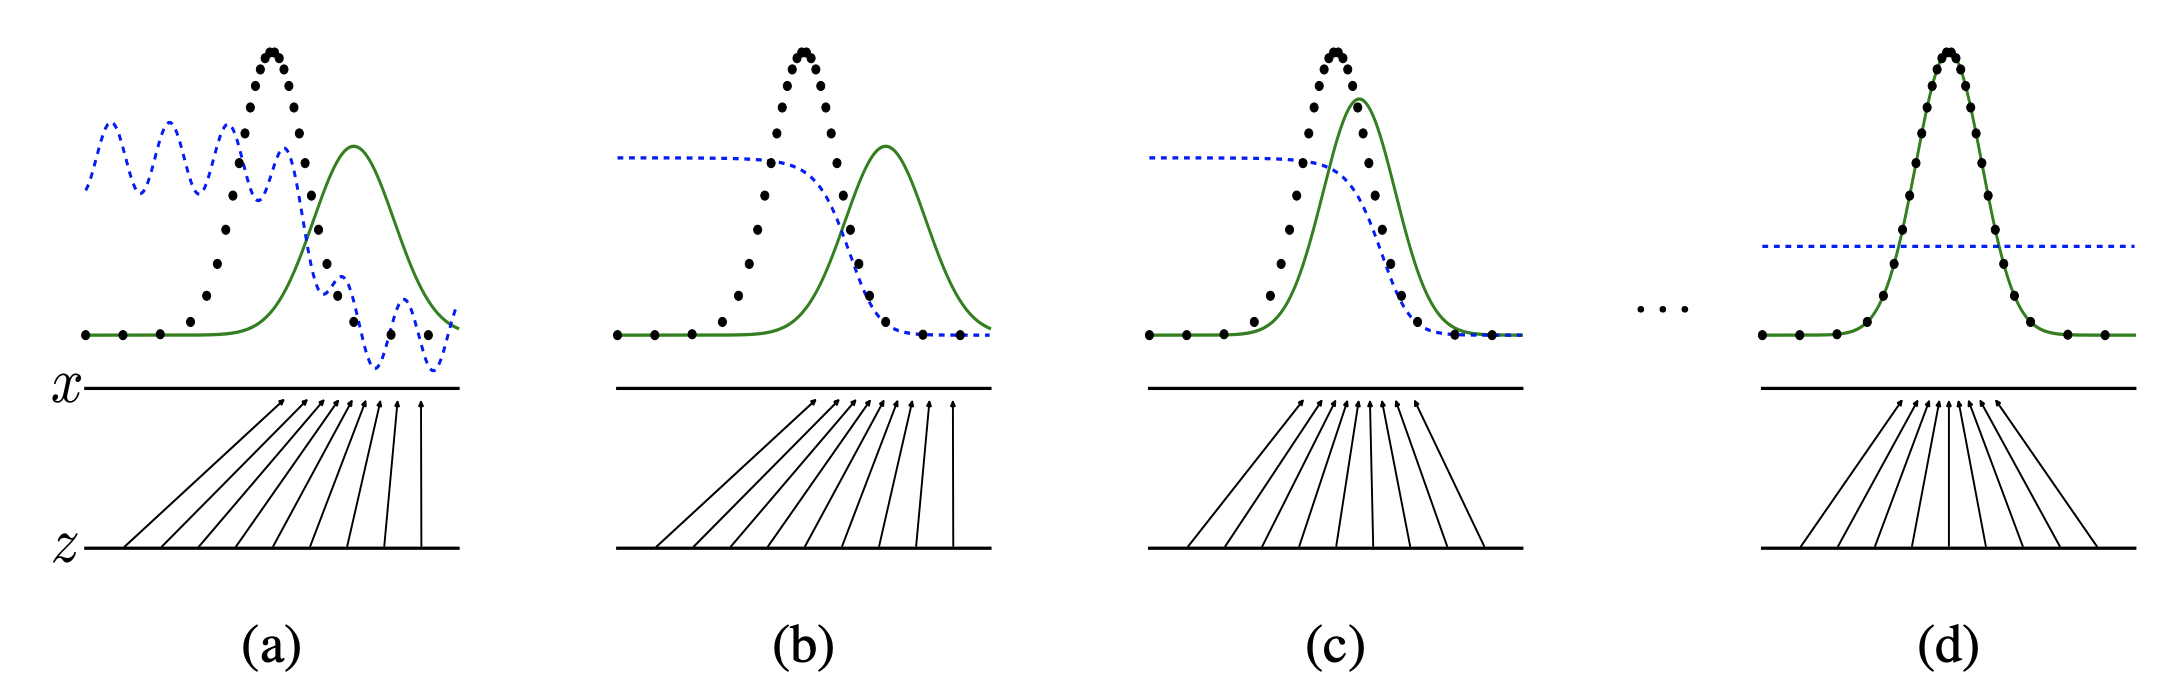
\includegraphics[width=1.0\linewidth]{figs/gan_1}
	\end{figure}
	\myfootnotewithlink{https://arxiv.org/abs/1406.2661}{Goodfellow I. J. et al. Generative Adversarial Networks, 2014}
\end{frame}
%=======
\begin{frame}{Recap of previous lecture}
\vspace{-0.3cm}
	\begin{block}{ELBO objective}
		\vspace{-0.5cm}
		\[
			 \mathcal{L} (\bphi, \btheta)  = \mathbb{E}_{q(\bz | \bx, \bphi)} \left[\log p(\bx | \bz, \btheta) - KL(\log q(\bz| \bx, \bphi) || p(\bz)) \right] \rightarrow \max_{\bphi, \btheta}.
		\]	
		\vspace{-0.5cm}
	\end{block}
	What is the problem to make the variational posterior model an \textbf{implicit} model? \\
	 We have to estimate density ratio (in KL term)
	\[
		r(\bx, \bz) = \frac{q_1(\bx, \bz)}{q_2(\bx, \bz)} = \frac{q(\bz| \bx, \bphi) \pi (\bx)}{p(\bz) \pi(\bx)} = \frac{D(\bx, \bz)}{1 - D(\bx, \bz)}.
	\] 
	\begin{block}{Adversarial Variational Bayes}
		\vspace{-0.6cm}
		\[
			\max_D \left[ \bbE_{\pi(\bx)} \bbE_{q(\bz | \bx, \bphi)} \log D(\bx, \bz) + \bbE_{\pi(\bx)} \bbE_{p(\bz)} \log (1 - D(\bx, \bz)) \right]
		\]
	\end{block}
	\myfootnotewithlink{https://arxiv.org/abs/1701.04722}{Mescheder L., Nowozin S., Geiger A. Adversarial variational bayes: Unifying variational autoencoders and generative adversarial networks, 2017}
\end{frame}
%=======
\begin{frame}{Outline}
	\tableofcontents
\end{frame}
%=======
\section{Wasserstein distance}
%=======
\begin{frame}{Informal theoretical results}
	\vspace{-0.3cm}
	\begin{itemize}
		\footnotesize
		\item Since $\bz$ usually has lower dimensionality compared to $\bx$, manifold $G(\bz, \btheta)$ has a measure 0 in $\bx$ space. Hence, support of $p(\bx | \btheta)$ lies on low-dimensional manifold.
		\item Distribution of real images $\pi(\bx)$ is also concentrated on a low dimensional manifold.
		\begin{figure}
			\centering
			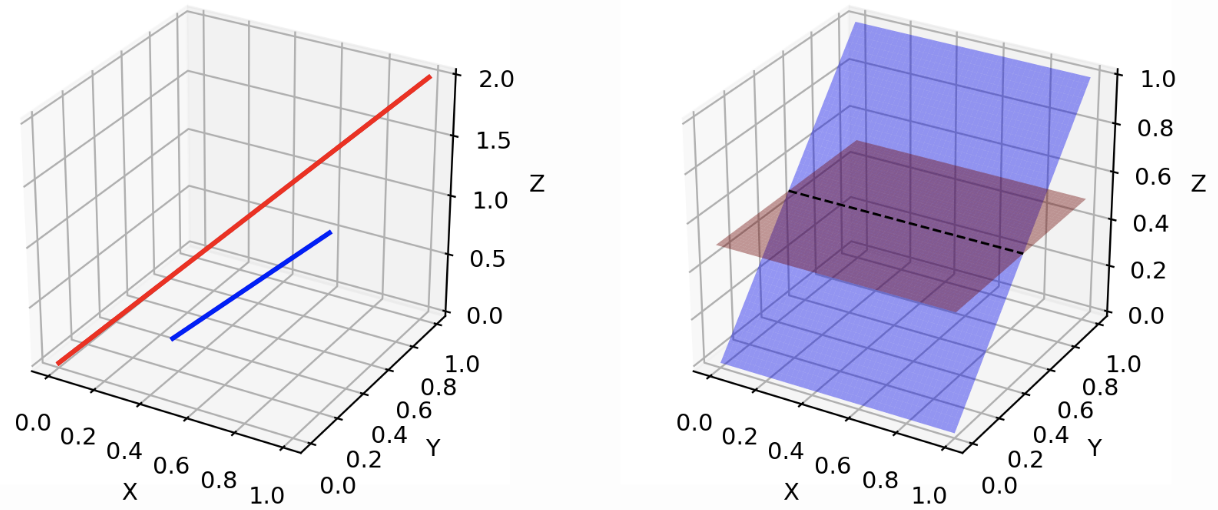
\includegraphics[width=0.5\linewidth]{figs/low_dim_manifold}
		\end{figure}
		\item If $\pi(\bx)$ and $p(\bx | \btheta)$ have disjoint supports, then there is a smooth optimal discriminator. We are not able to learn anything by backproping through it.
		\item For such low-dimensional disjoint manifolds
		\vspace{-0.2cm}
		\[
			KL(\pi || p) = KL(p || \pi) = \infty, \quad JSD(\pi || p) = \log 2
		\]
		\vspace{-0.7cm}
		\item Adding continuous noise to the inputs of the discriminator smoothes the distributions of the probability mass.
	\end{itemize}
	\myfootnote{\href{https://arxiv.org/abs/1904.08994}{Weng L. From GAN to WGAN, 2019} \\ 
	\href{https://arxiv.org/abs/1701.04862}{Arjovsky M., Bottou L. Towards Principled Methods for Training Generative Adversarial Networks, 2017}}
\end{frame}
%=======
\begin{frame}{Wasserstein distance (discrete)}
	A.k.a. \textbf{Earth Mover's distance}.
	The minimum cost of moving and transforming a pile of dirt in the shape of one probability distribution to the shape of the other distribution.
	\begin{figure}
		\centering
		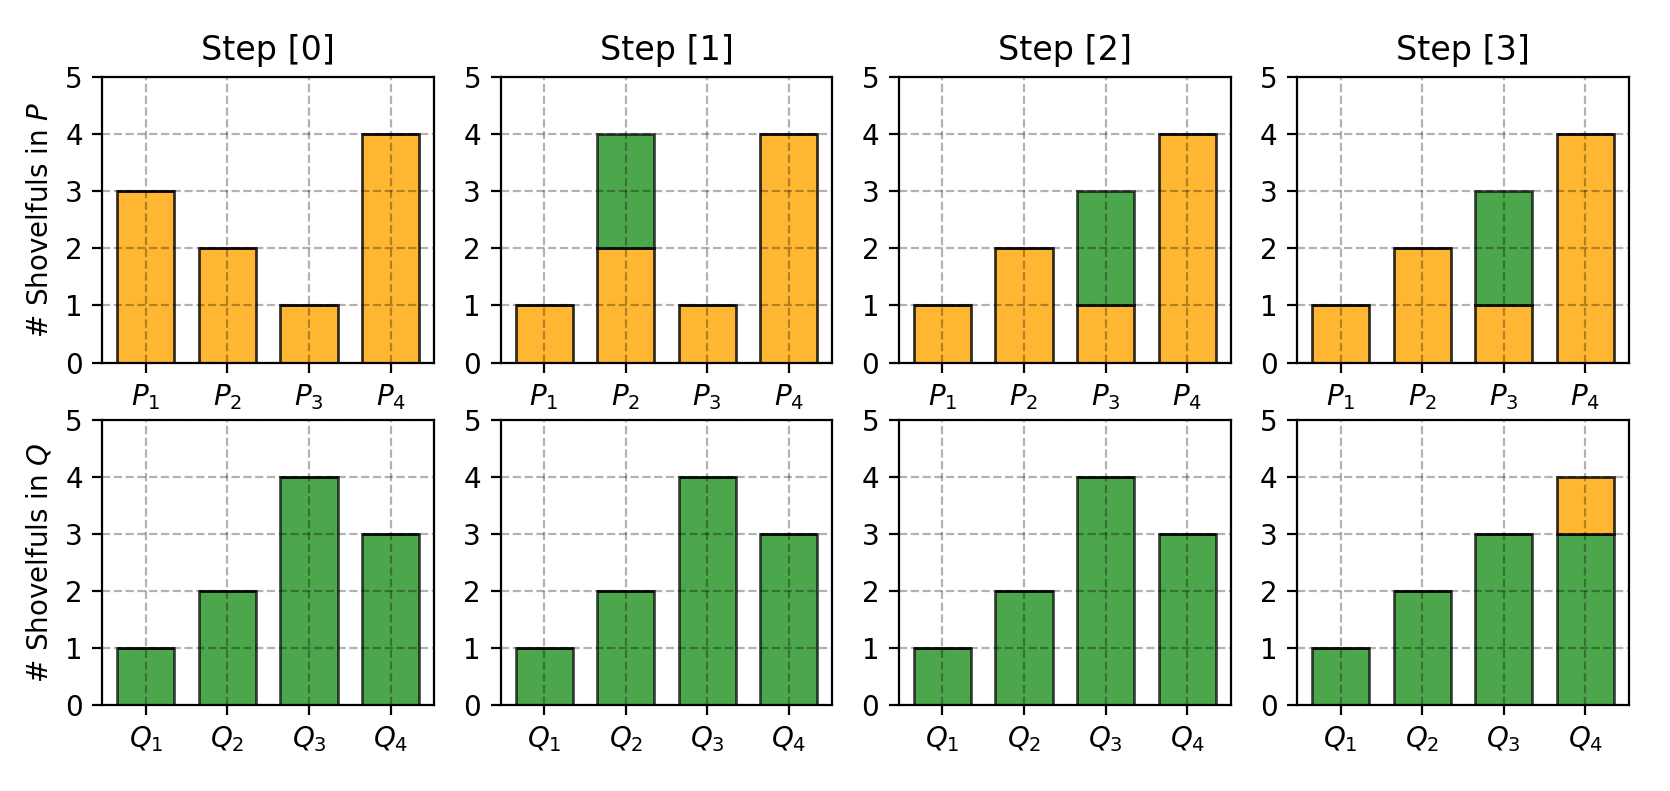
\includegraphics[width=.9\linewidth]{figs/EM_distance_discrete}
	\end{figure}
	\[
		W(P, Q) = 2 \text{(step 1)} + 2 \text{(step 2)} + 1 \text{(step 3)}  = 5
	\]
	\myfootnotewithlink{https://arxiv.org/abs/1904.08994}{Weng L. From GAN to WGAN, 2019} 
	
\end{frame}
%=======
\begin{frame}{Wasserstein distance (continuous)}
	\[
		W(\pi, p) = \inf_{\gamma \in \Gamma(\pi, p)} \bbE_{(\bx, \by) \sim \gamma} \| \bx - \by \| =  \inf_{{\color{olive}\gamma}\in {\color{teal}\Gamma(\pi, p)}} \int {\color{violet} \| \bx - \by \|} {\color{olive}\gamma (\bx, \by)} d \bx d \by
	\]
	\begin{itemize}
		\item ${\color{olive}\gamma (\bx, \by)}$ -- transportation plan (the amount of "dirt" that should be transported from point $\bx$ to point $\by$)
		\[
			 \int \gamma(\bx, \by) d \bx = p(\by); \quad \int \gamma(\bx, \by) d \by = \pi(\bx).
		\]
		\item ${\color{teal}\Gamma(\pi, p)}$ -- the set of all joint distributions $\gamma (\bx, \by)$ with marginals $\pi$ and $p$.
		\item ${\color{olive}\gamma(\bx, \by)}$ -- the amount, ${\color{violet} \| \bx - \by \|}$-- the distance.
	\end{itemize}
	{\color{gray}For better understanding of transportation plan function $\gamma$, try to write down the plan for previous discrete case.}
	\myfootnotewithlink{https://arxiv.org/abs/1701.07875}{Arjovsky M., Chintala S., Bottou L. Wasserstein GAN, 2017}
\end{frame}
%=======
\begin{frame}{Wasserstein distance vs KL vs JSD}
	
	\begin{minipage}[t]{0.48\columnwidth}
		\vspace{0.1cm}
		Consider 2d distributions
		\[
			\pi(x, y) = (0, U[0,1])
		\]	
		\[
			p(x, y | \theta) = (\theta, U[0, 1])
		\]
	\end{minipage}%
	\begin{minipage}[t]{0.52\columnwidth}
		\begin{figure}
			\centering
			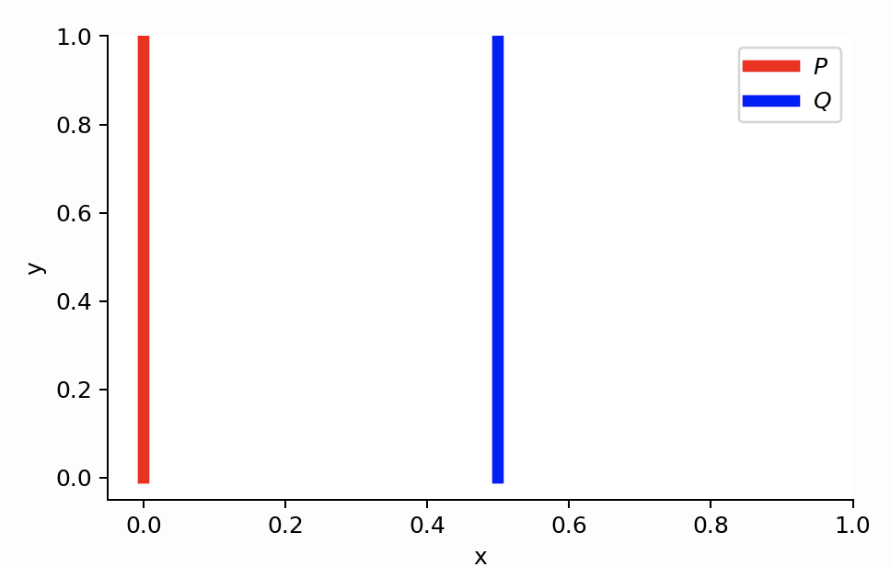
\includegraphics[width=0.8\linewidth]{figs/w_kl_jsd}
		\end{figure}
	\end{minipage}
	\begin{itemize}
		\footnotesize
		\item $\theta = 0$.
		Distributions are the same 
		\[
			KL(\pi || p) = KL(p || \pi) = JSD(p || \pi) = W(\pi, p) = 0
		\]
		\item $\theta \neq 0$
		\[
			KL(\pi || p) = \int_{U[0, 1]} 1 \log \frac{1}{0} d y = \infty = KL(p || \pi)
		\]
		\[
			JSD(\pi || p) = \frac{1}{2}\left( \int_{U[0, 1]}1 \log \frac{1}{1/2} dy + \int_{U[0, 1]}1 \log \frac{1}{1/2} dy \right) = \log 2
		\]
		\[
			W(\pi, p) = |\theta|
		\]
	\end{itemize}
	
	\myfootnote{\href{https://arxiv.org/abs/1904.08994}{Weng L. From GAN to WGAN, 2019} \\ 
	\href{https://arxiv.org/abs/1701.07875}{Arjovsky M., Chintala S., Bottou L. Wasserstein GAN, 2017}}
\end{frame}
%=======
\begin{frame}{Wasserstein distance vs KL vs JSD}
	\begin{block}{Theorem 1}
		Let $G(\bz, \btheta)$ be (almost) any feedforward neural network, and $p(\bz)$ a prior over $\bz$ such that $\bbE_{p(\bz)} \|\bz\| < \infty$. Then therefore $W(\pi, p)$ is continuous everywhere and differentiable almost everywhere.
	\end{block}
	\begin{block}{Theorem 2}
		Let $\pi$ be a distribution on a compact space $\cX$ and $\{p_t\}_{t=1}^\infty$ be a sequence of distributions on $\cX$. 
		\begin{align}
			KL(\pi || p_t) &\rightarrow 0 \, (\text{or }KL (p_t || \pi) \rightarrow 0) \\
			JSD(\pi || p_t) &\rightarrow 0 \\
			W(\pi || p_t) &\rightarrow 0
		\end{align}
		
		Then, considering limits as $t \rightarrow \infty$, (1) implies (2), (2) implies (3).
	\end{block}
	\myfootnotewithlink{https://arxiv.org/abs/1701.07875}{Arjovsky M., Chintala S., Bottou L. Wasserstein GAN, 2017}
\end{frame}
%=======
\section{Wasserstein GAN}
%=======
\begin{frame}{Wasserstein GAN}
	\begin{block}{Wasserstein distance}
		\vspace{-0.5cm}
		\[
			W(\pi || p) = \inf_{\gamma \in \Gamma(\pi, p)} \bbE_{(\bx, \by) \sim \gamma} \| \bx - \by \| =  \inf_{\gamma \in \Gamma(\pi, p)} \int \| \bx - \by \| \gamma (\bx, \by) d \bx d \by
		\]
		\vspace{-0.3cm}
	\end{block}
	The infimum across all possible joint distributions in $\Gamma(\pi, p)$ is intractable.
	\begin{block}{Theorem (Kantorovich-Rubinstein duality)}
		\vspace{-0.3cm}
		\[
			W(\pi || p) = \frac{1}{K} \max_{\| f \|_L \leq K} \left[ \bbE_{\pi(\bx)} f(\bx)  - \bbE_{p(\bx)} f(\bx)\right],
		\]
		where $\| f \|_L \leq K$ are $K-$Lipschitz continuous functions ($f: \cX \rightarrow \bbR$)
		\vspace{-0.2cm}
		\[
			|f(\bx_1) - f(\bx_2)| \leq K \| \bx_1 - \bx_2 \|, \quad \text{for all } \bx_1, \bx_2 \in \cX.
		\]
		\vspace{-0.5cm}
	\end{block}
	Now we need only samples to get Monte Carlo estimate for $W(\pi || p)$.

	\myfootnotewithlink{https://arxiv.org/abs/1701.07875}{Arjovsky M., Chintala S., Bottou L. Wasserstein GAN, 2017}
\end{frame}
%=======
\begin{frame}{Wasserstein GAN}
	\begin{block}{Theorem (Kantorovich-Rubinstein duality)}
		\[
		W(\pi || p) = \frac{1}{K} \max_{\| f \|_L \leq K} \left[ \bbE_{\pi(\bx)} f(\bx)  - \bbE_{p(\bx)} f(\bx)\right],
		\]
	\end{block}
	\begin{itemize}
		\item Now we have to ensure that $f$ is $K$-Lipschitz continuous.
		\item Let $f(\bx, \bphi)$ be a feedforward neural network parametrized by~$\bphi$.
		\item If parameters $\bphi$ lie in a compact set $\boldsymbol{\Phi}$ then $f(\bx, \bphi)$ will be $K$-Lipschitz continuous function. 
		\item Let the parameters be clamped to a fixed box $\boldsymbol{\Phi} \in [-c, c]^d$ (e.x. $c = 0.01$) after each gradient update.
	\end{itemize}
	\begin{multline*}
		K \cdot W(\pi || p) = \max_{\| f \|_L \leq K} \left[ \bbE_{\pi(\bx)} f(\bx)  - \bbE_{p(\bx)} f(\bx)\right] \geq \\  \geq \max_{\bphi \in \boldsymbol{\Phi}} \left[ \bbE_{\pi(\bx)} f(\bx, \bphi)  - \bbE_{p(\bx)} f(\bx, \bphi )\right]
	\end{multline*}
	
	\myfootnotewithlink{https://arxiv.org/abs/1701.07875}{Arjovsky M., Chintala S., Bottou L. Wasserstein GAN, 2017}
\end{frame}
%=======
\begin{frame}{Wasserstein GAN}
	\begin{block}{Standard GAN objective}
		\vspace{-0.2cm}
		\[
		\min_{\btheta} \max_{\bphi} \bbE_{\pi(\bx)} \log D(\bx, \bphi) + \bbE_{p(\bz)} \log (1 - D(G(\bz, \btheta), \bphi))
		\]
		\vspace{-0.2cm}
	\end{block}
	\begin{block}{WGAN objective}
		\vspace{-0.6cm}
		\[
		\min_{\btheta} W(\pi || p) \approx \min_{\btheta} \max_{\bphi \in \boldsymbol{\Phi}} \left[ \bbE_{\pi(\bx)} f(\bx, \bphi)  - \bbE_{p(\bz)} f(G(\bz, \btheta), \bphi )\right].
		\]
		\vspace{-0.3cm}
	\end{block}
	\begin{itemize}
		\item Discriminator $D$ is similar to the function $f$, but not the same (it is not a classifier anymore). In the WGAN model, function~$f$ is usually called $\textbf{critic}$.
		\item \textit{"Weight clipping is a clearly terrible way to enforce a Lipschitz constraint"}. If the clipping parameter $c$ is too large, it is hard to train the critic till optimality. If the clipping parameter $c$ is too small, it could lead to vanishing gradients.
	\end{itemize}
	
	\myfootnotewithlink{https://arxiv.org/abs/1701.07875}{Arjovsky M., Chintala S., Bottou L. Wasserstein GAN, 2017}
\end{frame}
%=======
\begin{frame}{Wasserstein GAN}
	\begin{minipage}[t]{0.6\columnwidth}
		\begin{itemize}
			\item WGAN has non-zero gradients for disjoint supports.
			\item $JSD(\pi || p)$ correlates poorly with the sample quality. Stays constast nearly maximum value $\log 2 \approx 0.69$.
			\item $W(\pi || p)$ is highly correlated with the sample quality. 
		\end{itemize}
	\end{minipage}%
	\begin{minipage}[t]{0.4\columnwidth}
		\begin{figure}
			\centering
			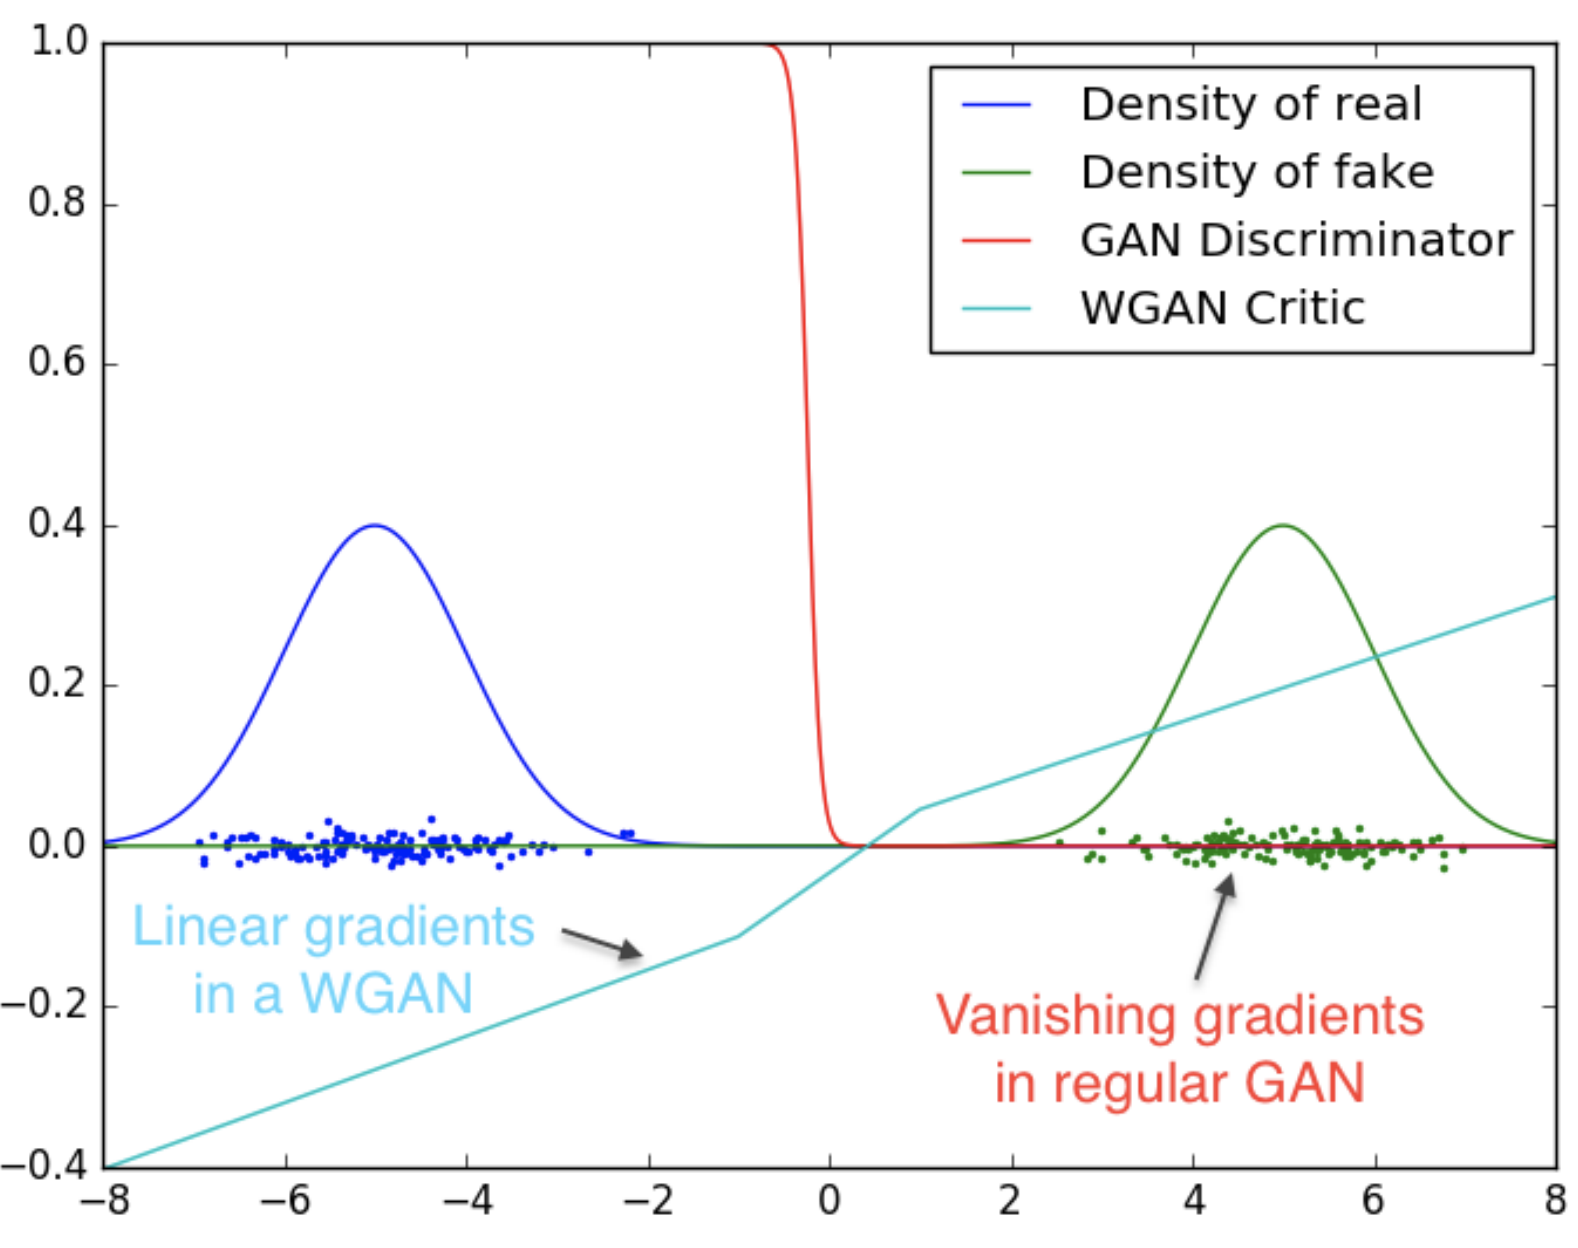
\includegraphics[width=\linewidth]{figs/wgan_toy}
		\end{figure}
	\end{minipage}
	\begin{minipage}[t]{0.5\columnwidth}
		\begin{figure}
			\centering
			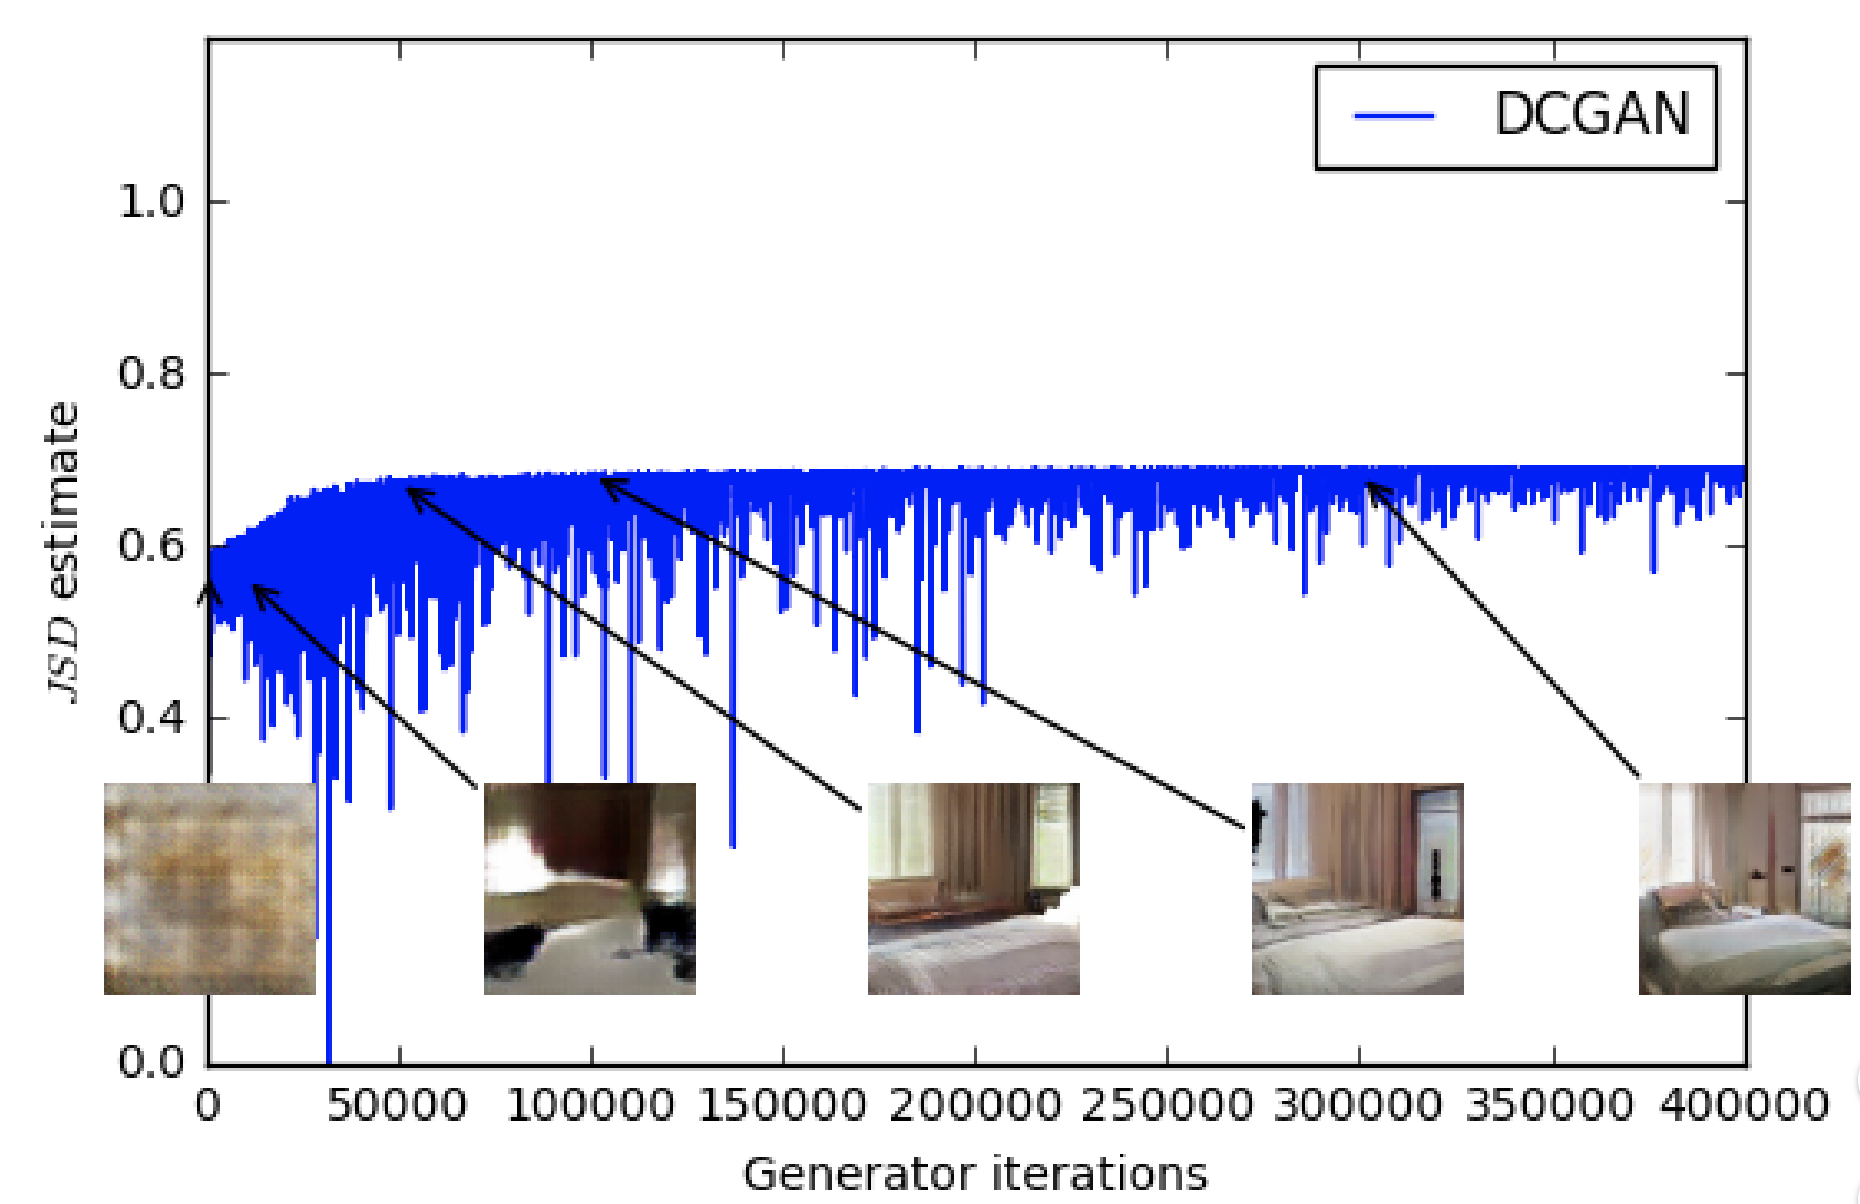
\includegraphics[width=1.0\linewidth]{figs/dcgan_quality}
		\end{figure}
	\end{minipage}%
	\begin{minipage}[t]{0.5\columnwidth}
		\begin{figure}
			\centering
			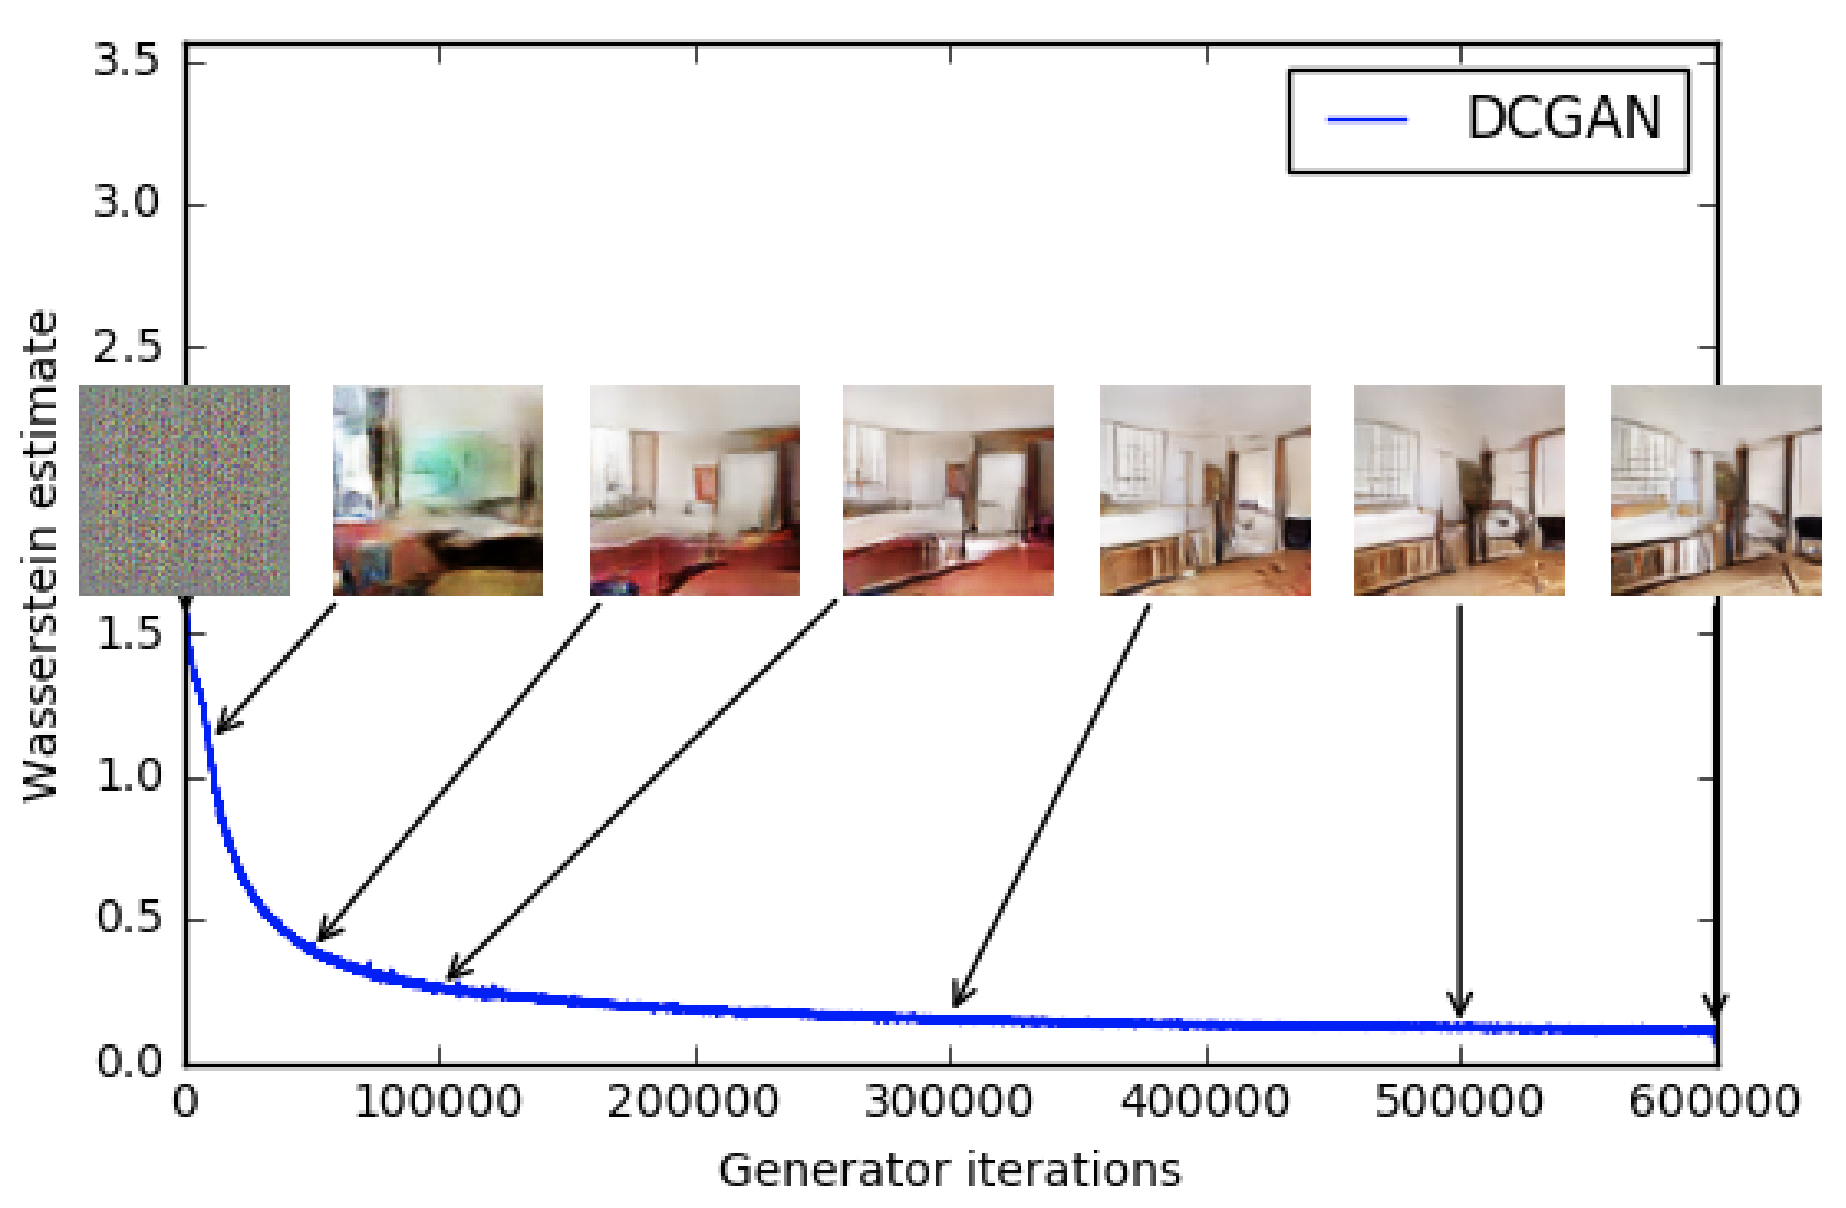
\includegraphics[width=1.0\linewidth]{figs/wgan_quality}
		\end{figure}
	\end{minipage}
	
	\myfootnotewithlink{https://arxiv.org/abs/1701.07875}{Arjovsky M., Chintala S., Bottou L. Wasserstein GAN, 2017}
\end{frame}
%=======
\section{Lipschitzness of Wasserstein GAN critic}
%=======
\subsection{WGAN with Gradient Penalty}
%=======
\begin{frame}{Wasserstein GAN with Gradient Penalty}
	\vspace{-0.2cm}
	\begin{figure}
		\centering
		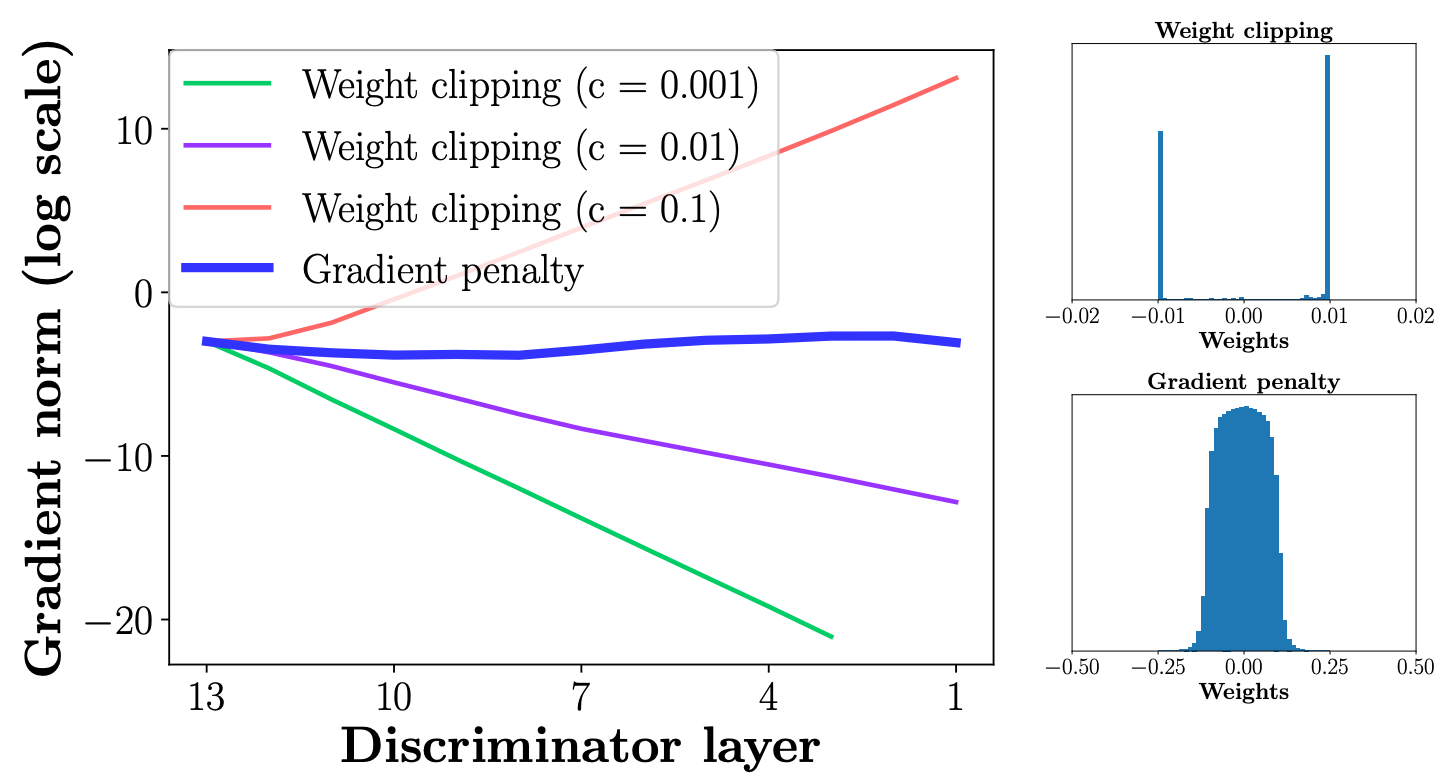
\includegraphics[width=0.9\linewidth]{figs/wgan_gp_weights}
	\end{figure}
	\vspace{-0.2cm} 
	
	\begin{block}{Weight clipping analysis}
		\begin{itemize}
			\item The gradients either grow or decay exponentially.
			\item Gradient penalty makes the gradients more stable.
		\end{itemize}
	\end{block}
	\myfootnotewithlink{https://arxiv.org/abs/1704.00028}{Gulrajani I. et al. Improved Training of Wasserstein GANs, 2017}
\end{frame}
%=======
\begin{frame}{Wasserstein GAN with Gradient Penalty}
	\begin{block}{Theorem}
		Let $\pi(\bx)$ and $p(\bx)$ be two distribution in $\cX$, a compact metric space. Let $\gamma$ be the optimal transportation plan between $\pi(\bx)$ and $p(\bx)$. Then
		\begin{enumerate}
			\item there is 1-Lipschitz function $f^*$ which is the optimal solution of 
			\[
				\max_{\| f \|_L \leq 1} \left[ \bbE_{\pi(\bx)} f(\bx)  - \bbE_{p(\bx)} f(\bx)\right].
			\]
			\item if $f^*$ is differentiable, $\gamma(\by = \bz) = 0$ and $\hat{\bx}_t = t \by + (1 - t) \bz$ with $\by \sim \pi(\bx)$, $\bz \sim p(\bx | \btheta)$, $t \in [0, 1]$ it holds that
			\[
				\bbP_{(\by, \bz) \sim \gamma} \left[ \nabla f^*(\hat{\bx}_t) = \frac{\bz - \hat{\bx}_t}{\| \bz - \hat{\bx}_t \|} \right] = 1.
			\]
		\end{enumerate}
	\end{block}
	\vspace{-0.5cm}
	\begin{block}{Corollary}
		$f^*$ has gradient norm 1 almost everywhere under $\pi(\bx)$ and $p(\bx)$.
	\end{block}

	\myfootnotewithlink{https://arxiv.org/abs/1704.00028}{Gulrajani I. et al. Improved Training of Wasserstein GANs, 2017}
\end{frame}
%=======
\begin{frame}{Wasserstein GAN with Gradient Penalty}
	A differentiable function is 1-Lipschtiz if and only if it has gradients with norm at most 1 everywhere.
	\begin{block}{Gradient penalty}
		\vspace{-0.3cm}
		\[
			W(\pi || p) = \underbrace{\bbE_{\pi(\bx)} f(\bx)  - \bbE_{p(\bx)} f(\bx)}_{\text{original critic loss}} + \lambda \underbrace{\bbE_{U[0, 1]} \left[ \left( \| \nabla f(\hat{\bx}) \|_2 - 1 \right) ^ 2\right]}_{\text{gradient penalty}},
		\]
		\vspace{-0.3cm}
	\end{block}
	\begin{itemize}
		\item Samples $\hat{\bx}_t = t \by + (1 - t) \bz$ with $t \in [0, 1]$ are uniformly sampled along straight lines between pairs of points: $\by$ from the data distribution $\pi(\bx)$ and $\bz$ from the generator distribution $p(\bx | \btheta)$.
		\item Enforcing the unit gradient norm constraint everywhere is intractable, it turns out to be sifficient to enforce it only along these straight lines.
	\end{itemize}

	\myfootnotewithlink{https://arxiv.org/abs/1704.00028}{Gulrajani I. et al. Improved Training of Wasserstein GANs, 2017}
\end{frame}
%=======
\subsection{Spectral Normalization GAN}
%=======
\begin{frame}{Spectral Normalization GAN}
	\begin{block}{Definition}
		$\| \bA \|_2$ is a \textit{spectral norm} of matrix $\bA$:
		\[
			\| \bA \|_2 = \max_{\bh \neq 0} \frac{\|\bA \bh\|_2}{\|\bh\|_2} = \max_{\|\bh\|_2 \leq 1} \| \bA \bh \|_2 = \sqrt{\lambda_{\text{max}}(\bA^T \bA)},
		\]
		where $\lambda_{\text{max}}(\bA^T \bA)$ is the largest eigenvalue value of $\bA^T \bA$.
	\end{block}
	\begin{block}{Statement 1}
		if $\mathbf{g}$ is a K-Lipschitz vector function then 
		\[
			\| \mathbf{g} \|_L \leq K = \sup_\bx \| \nabla \mathbf{g}(\bx) \|_2.
		\]
		\vspace{-0.7cm}
	\end{block}
	\begin{block}{Statement 2}
		Lipschitz norm of superposition is bounded above by product of Lipschitz norms
		\vspace{-0.2cm}
		\[
			\| \mathbf{g}_1 \circ \mathbf{g}_2 \|_L \leq \| \mathbf{g}_1 \|_L \cdot \| \mathbf{g}_2\|_L
		\]
	\end{block}
	\myfootnotewithlink{https://arxiv.org/abs/1802.05957}{Miyato T. et al. Spectral Normalization for Generative Adversarial Networks, 2018}
\end{frame}
%=======
\begin{frame}{Spectral Normalization GAN}
	Let consider the critic $f(\bx, \bphi)$ of the following form:
	\[
		f(\bx, \bphi) = \bW_{K+1} \sigma_K (\bW_K \sigma_{K-1}(\dots \sigma_1(\bW_1 \bx) \dots)).
	\]
	This feedforward network is a superposition of simple functions.
	\begin{itemize}
		\item $\sigma_k$ is a pointwise nonlinearities. We assume that $\| \sigma_k \|_L = 1$ (it holds for ReLU).
		\item $\mathbf{g}(\bx) = \bW^T \bx$ is a linear transformation ($\nabla \mathbf{g}(\bx) = \bW$).
		\[
			\| \mathbf{g} \|_L \leq \sup_\bx \| \nabla \mathbf{g}(\bx)\|_2 = \| \bW \|_2.
		\]
	\end{itemize}
	\vspace{-0.4cm}
	\begin{block}{Critic spectral norm}
		\vspace{-0.4cm}
		\[
			\| f \|_L \leq \| \bW_{K+1}\|_2 \cdot \prod_{k=1}^K  \| \sigma_k \|_L \cdot \| \bW_k \|_2 = \prod_{k=1}^{K+1} \|\bW_k\|_2.
		\]
		\vspace{-0.2cm}
	\end{block}
	If we replace the weights in the critic $f(\bx, \bphi)$ by $\bW^{SN}_k = \bW_k / \|\bW_k\|_2$, we will get $\| f\|_L \leq 1.$ \\
	
	\myfootnotewithlink{https://arxiv.org/abs/1802.05957}{Miyato T. et al. Spectral Normalization for Generative Adversarial Networks, 2018}
\end{frame}
%=======
\begin{frame}{Spectral Normalization GAN}
	How to compute $ \| \bW \|_2 = \sqrt{\lambda_{\text{max}}(\bW^T \bW)}$? \\
	We are not able to apply SVD at each iteration.
	 \begin{block}{Power iteration (PI) method}
	 	\vspace{-0.2cm}
	 	\begin{itemize}
	 		\item $\bu_0$ -- random vector.
	 		\item for $m = 0, \dots, M - 1$: ($M$ is a fixed number of steps)
	 		\vspace{-0.3cm}
	 		\[
	 			\bv_{m+1} = \frac{\bW^T \bu_{m}}{\| \bW^T \bu_{m} \|}, \quad \bu_{m+1} = \frac{\bW \bv_{m+1}}{\| \bW \bv_{m+1} \|}.
	 		\]
	 		\item approximate the spectral norm
	 		\vspace{-0.3cm}
	 		\[
	 			\| \bW \|_2 = \sqrt{\lambda_{\text{max}}(\bW^T \bW)} \approx \bu_{M}^T \bW \bv_{M}.
	 		\]
	 	\end{itemize}
	 \end{block}
	 \vspace{-0.5cm}
 	\begin{block}{SNGAN gradient update}
 		\begin{itemize}
 			\item Apply PI method to get approximation of spectral norm.
 			\item Normalize weights $\bW^{SN}_k = \bW_k / \|\bW_k\|_2$.
 			\item Apply gradient rule to $\bW$.
 		\end{itemize}
 	\end{block}

	\myfootnotewithlink{https://arxiv.org/abs/1802.05957}{Miyato T. et al. Spectral Normalization for Generative Adversarial Networks, 2018}
\end{frame}
%=======
\begin{frame}{Summary}
	\begin{itemize}
		\item KL and JS divergences work poorly as model objective in the case of disjoint supports.
		\vfill
		\item Earth-Mover distance is a more appropriate objective function for distribution matching problem.	
		\vfill
		\item Kantorovich-Rubinstein duality gives the way to calculate the EM distance using only samples.
		\vfill
		\item Wasserstein GAN uses Kantorovich-Rubinstein duality for getting Earth Mover distance as model objective.
		\vfill
		\item Weight clipping is a terrible way to enforce Lipschitzness. Gradient Penalty adds regularizer to loss that uses neccessary conditions for optimal critic.
		\vfill
		\item Spectral normalization is a weight normalization technique to enforce Lipshitzness, which is helpful for generator and critic.
	\end{itemize}
\end{frame}
%=======
\end{document} 